\documentclass[12pt,letterpaper]{article}
\usepackage[margin=1in]{geometry}
\usepackage[intlimits]{amsmath}
\usepackage{graphicx}
\usepackage{fancybox}
\usepackage{ifthen}
\usepackage{url}
\usepackage{lscape,afterpage}
\usepackage{xspace}
\usepackage{epstopdf} 
\usepackage{subcaption}
\graphicspath{{Figures/}}
\begin{document}
\title{Technical Note: $^{11}$C Spallation Production Measurement}
\author{Hasung Song}
\maketitle
\begin{abstract}
	This technical note describes the $^{11}$C measurement in KLZ and how the rate is extracted.
\end{abstract}

\subsection*{Spallation Event Selection}
\begin{itemize}
	\item Standard FBE muon selection cuts
	\item Standard MoGURA neutron selection cuts
	\item Neutron Shower Cuts ($N_n=1$)
	\item XeLS $^{11}$C Candidate cuts
	\begin{itemize}
		\item Energy Range  : 1.0-1.6 MeV
		\item Radius : 0-160 cm
		\item dT : 100-18,000 s (5 hours)
	\end{itemize}
	\item KamLS $^{11}$C Candidate cuts
	\begin{itemize}
		\item Energy Range  : 1.4-2.4 MeV
		\item Radius : 220-350 cm
		\item dT : 100-18,000 s (5 hours)
	\end{itemize}
	\item $dR$ Cut : $<80$ cm
\end{itemize}

\subsection*{Fit to $dT$}
dT of muon-event pairs where the neutron shower contained 1 observed neutron is shown in Figure \ref{fig:dT_fits}.
\begin{figure}[ht]
	\centering
	\subcaptionbox{XeLS\label{fig:dT_XeLS}}[0.45\textwidth]{
		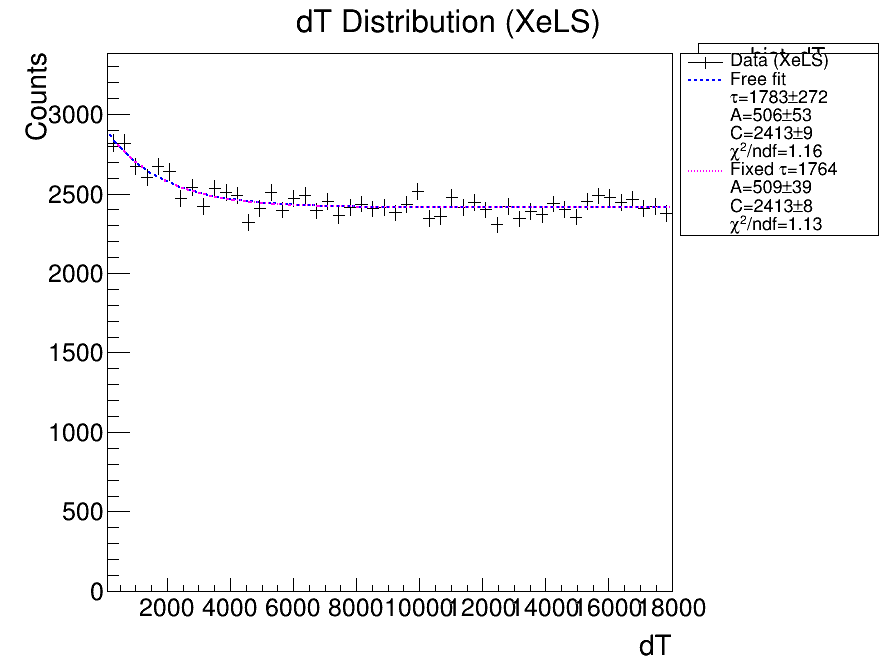
\includegraphics[width=0.45\textwidth]{dT_distribution_allcuts_XeLS.png}}
	\hfill
	\subcaptionbox{KamLS\label{fig:dT_KamLS}}[0.45\textwidth]{
		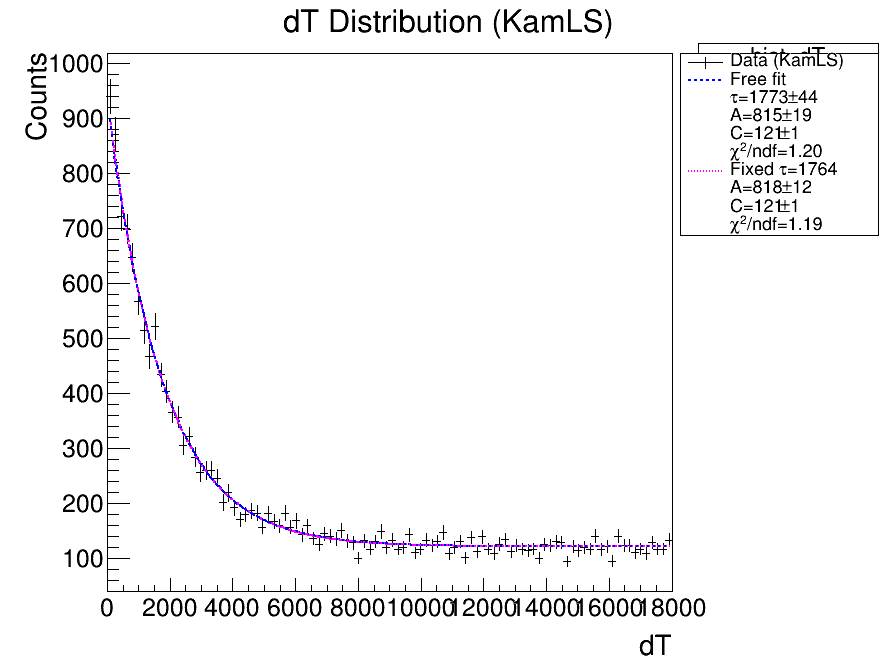
\includegraphics[width=0.45\textwidth]{dT_distribution_allcuts_KamLS.png}}
	\caption{dT of muon-event pairs where the neutron shower contained 1 observed neutron.}
	\label{fig:dT_fits}
\end{figure}

\subsection*{Rate Calculation}
The calculation of expected number of detected, selected, and correlated $^{11}$C-$\mu$ pairs.
\begin{equation}
	I_{C11} = Y_{C11}\times E_{FBE} \times (1-dt_{MoG}) \times P_n(1|^{11}C_{spall}) \times \epsilon_{dR} \times \epsilon_{dT} \times \epsilon_{FV} \times \epsilon_{E}
\end{equation}
\begin{itemize}
	\item $I_{C11}$: Integral of the exponential component of the fit, "Observed $\mu-^{11}$C pairs" $[events]$
	\item $Y_{C11}$: Production rate of $^{11}$C in KamLS, XeLS \textbf{final result} $[events/kton\cdot days]$
	\item $E_{FBE}$: Exposure, Livetime : $[kton\cdot days]$
	\begin{itemize}
		\item Go through FBE runs and sum up muon veto/detector deadtimes, integrate FV.
	\end{itemize}
	\item $dt_{MoG}$: MoGURA Deadtime Fraction: [unitless]
	\begin{itemize}
		\item simply scale up based on the deadtime since muons that occur during deadtime will not be able to create accurate pairs.
		\item Have to go through the MoGURA/FBE runs and check for overlap.
	\end{itemize}
	\item $P_n(1|^{11}C_{spall})$: Neutron Production : How many muons that create $^{11}$C create exactly 1 \textbf{observed} neutron [unitless]
	\begin{itemize}
		\item Muons that create $^{11}$C and create $1+$ neutrons, some fraction of those have only one detected (Toy MC calculation using Neutron Tagging Efficiency and FLUKA simulated neutron yield)
		\item Can estimate the rate of muons creating other isotopes, should be ~1\% of $^{11}$C production in the analysis dT range.
	\end{itemize}
	\item $\epsilon_{dR}$: dR cut efficiency (from FLUKA tuned with $^{11}$C), for each data period [unitless]
	\item $\epsilon_{dT}$: dT $>100$s cut efficiency (from known $^{11}$C half-life) [unitless]
	\item $\epsilon_{FV}$: Fiducial Volume Cut Efficiency (KLG4Sim) [unitless]
	\item $\epsilon_{E}$: Energy Cut Efficiency (KLG4Sim) [unitless]
\end{itemize}
Simply solve for $Y_{C11}$:
\begin{equation}
	Y_{C11} = \frac{I_{C11}}{E_{FBE} \times (1-dt_{MoG}) \times P_n(1|^{11}C_{spall}) \times \epsilon_{dR} \times \epsilon_{dT} \times \epsilon_{FV} \times \epsilon_{E}}
\end{equation}
\subsection*{Systematic Errors}
\begin{itemize}
	\item $A_{C11}$, exponential amplitude, fit uncertainty : $A_{C11}=509\pm39$, $\frac{39}{504}=7.7\%$
	\item Exposure Uncertainty, from $0\nu$ analysis uncertainty $\sim 4\%$
	\begin{itemize}
		\item 4\% uncertainty stated for uncertainty in xenon exposure, mainly driven by FV uncertainty, similar for Carbon?
	\end{itemize}
	\item Neutron Tagging Efficiency Error: $74.5\%\pm0.4\%$
	\item FLUKA simulation Systematic : dR Cut, Neutron Production
	\item FLUKA simulation Statistical (insignificant)
	\item Energy Scale Uncertainty : (use 1 sigma of kB, R contour)
\end{itemize}

\subsection*{Result}


\end{document}